\documentclass{bmstu}

\bibliography{biblio}

\begin{document}

\makereporttitle
    {Информатика и системы управления}
    {Программное обеспечение ЭВМ и информационные технологии}
    {лабораторной работе №1}
    {Архитектура ЭВМ}
    {Изучение принципов работы микропроцессорного ядра RISC-V}
    {17}
    {М.~А.~Семенчук/ИУ7-55Б}
    {А.~Ю.~Попов}

\newcommand{\mychapter}[2]{
    \setcounter{chapter}{#1}
    \setcounter{section}{0}
    \chapter*{#2}
    \addcontentsline{toc}{chapter}{#2}
}

\maketableofcontents

\chapter*{Введение}

Основной целью работы является ознакомление с принципами функционирования, построения и особенностями архитектуры суперскалярных конвейерных микропроцессоров. Дополнительной целью работы является знакомство с принципами проектирования и верификации сложных цифровых устройств с использованием языка описания аппаратуры SystemVerilog и ПЛИС.

Для достижения поставленных целей в настоящей лабораторной работе используется синтезируемое описание микропроцессорного ядра Taiga\footnote{https://gitlab.com/sfu-rcl/Taiga, авторы - Eric Matthews,  Lesley Shannon}, реализующего систему команд RV32I семейства RISC-V. Данное описание выполнено на языке описания аппаратуры SystemVerilog.

В ходе лабораторной работы используется средство моделирования MentorGraphics Modelsim для моделирования работы исследуемого микропроцессора в процессе выполнения программы и наблюдения формы внутренних сигналов.
\chapter{Задание №1}

\section{Текст программы по индивидуальному варианту}

\lstinputlisting[caption=Текст программы по индивидуальному варианту, frame=single, numbers=left]{code/prog.s}

\section{Дизассемблерный листинг кода программы}

\lstinputlisting[caption=Дизассемблерный листинг кода программы, frame=single, numbers=left]{code/disasm}

\section{Псевдокод, поясняющий работу программы}

\lstinputlisting[language=C, caption="Псевдокод поясняющий работу программы", frame=single, numbers=left]{code/prog.c}

Приведенный код находит \textbf{максимальный} элемент массива, используя попарное сравнение элементов. Следовательно, после работы программы регистр \textbf{x31} будет содержать число \textbf{9}.
\mychapter{2}{Задание №2}

\begin{center}
\centering 
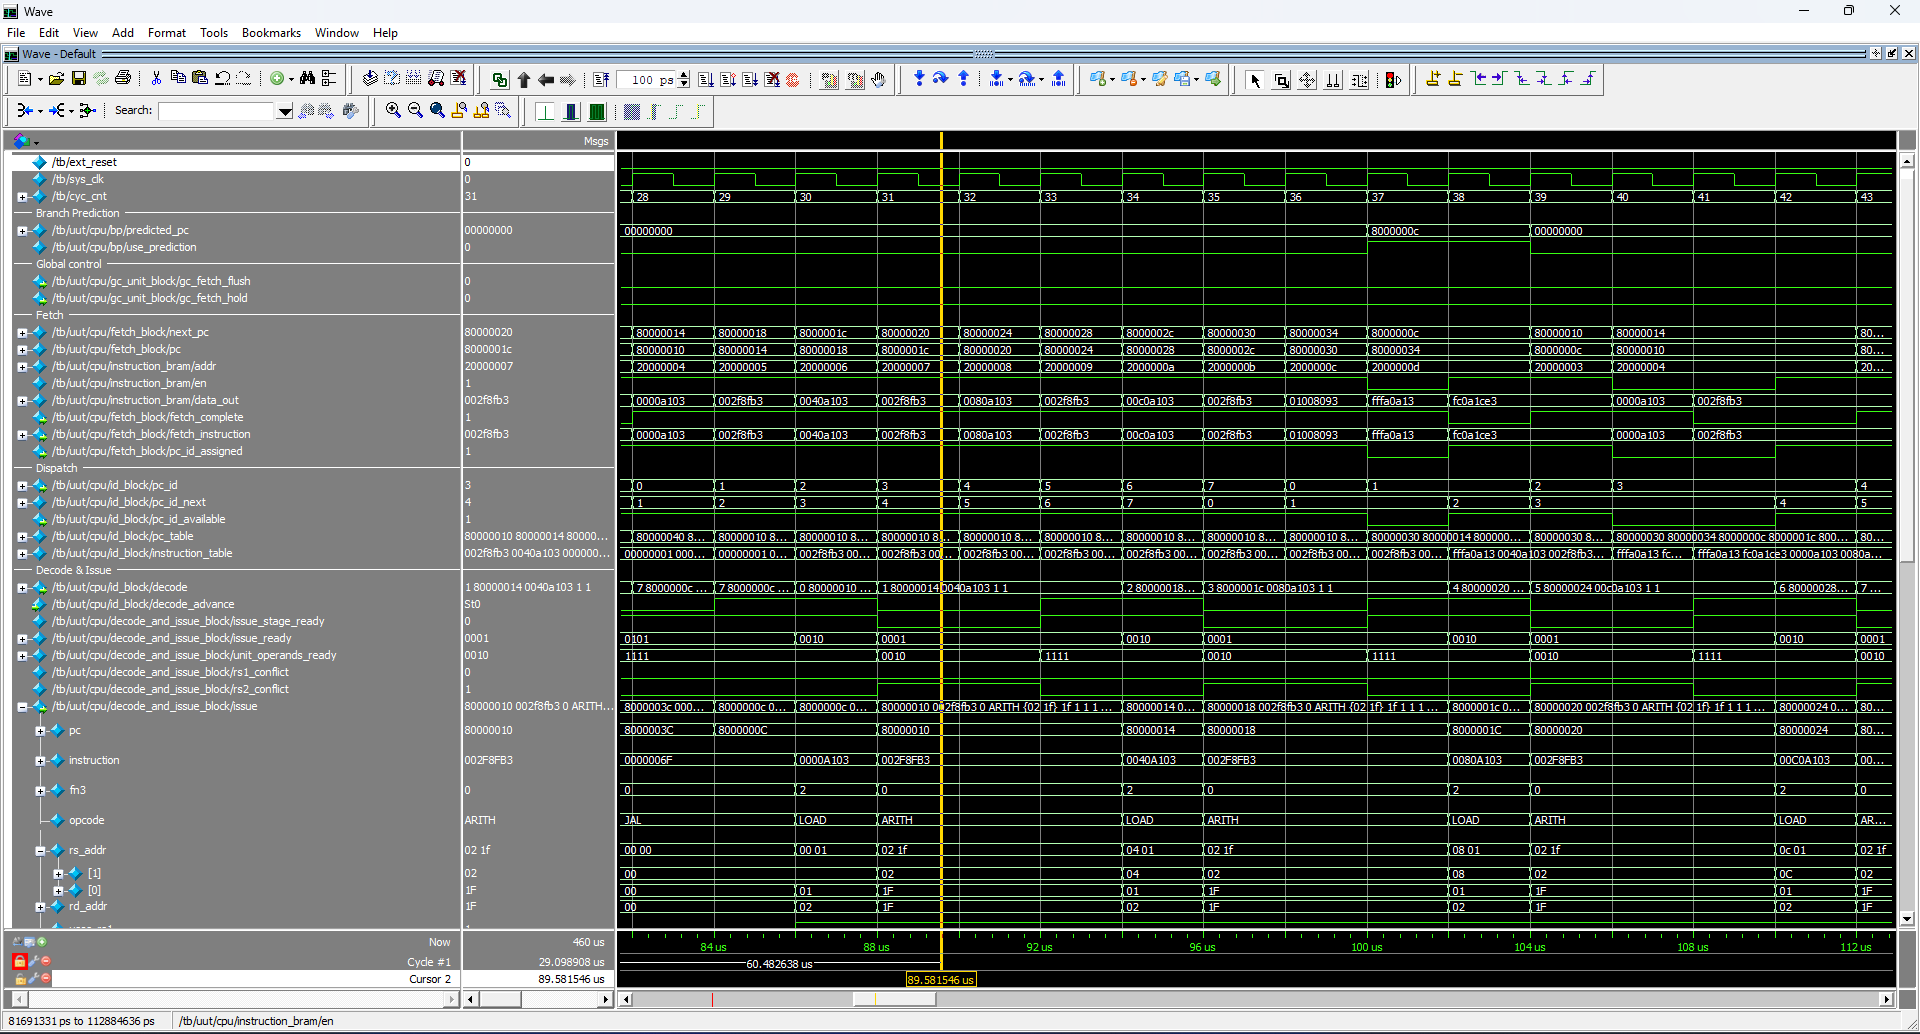
\includegraphics[scale=0.25]{images/02-F_ID.png}
 \captionof{figure}{Временная диаграмма выполнения стадий выборки и диспетчеризации команды с \textbf{адресом 80000020 на 2-й итерации}}
\end{center}
\mychapter{3}{Задание №3}

\begin{center}
\centering 
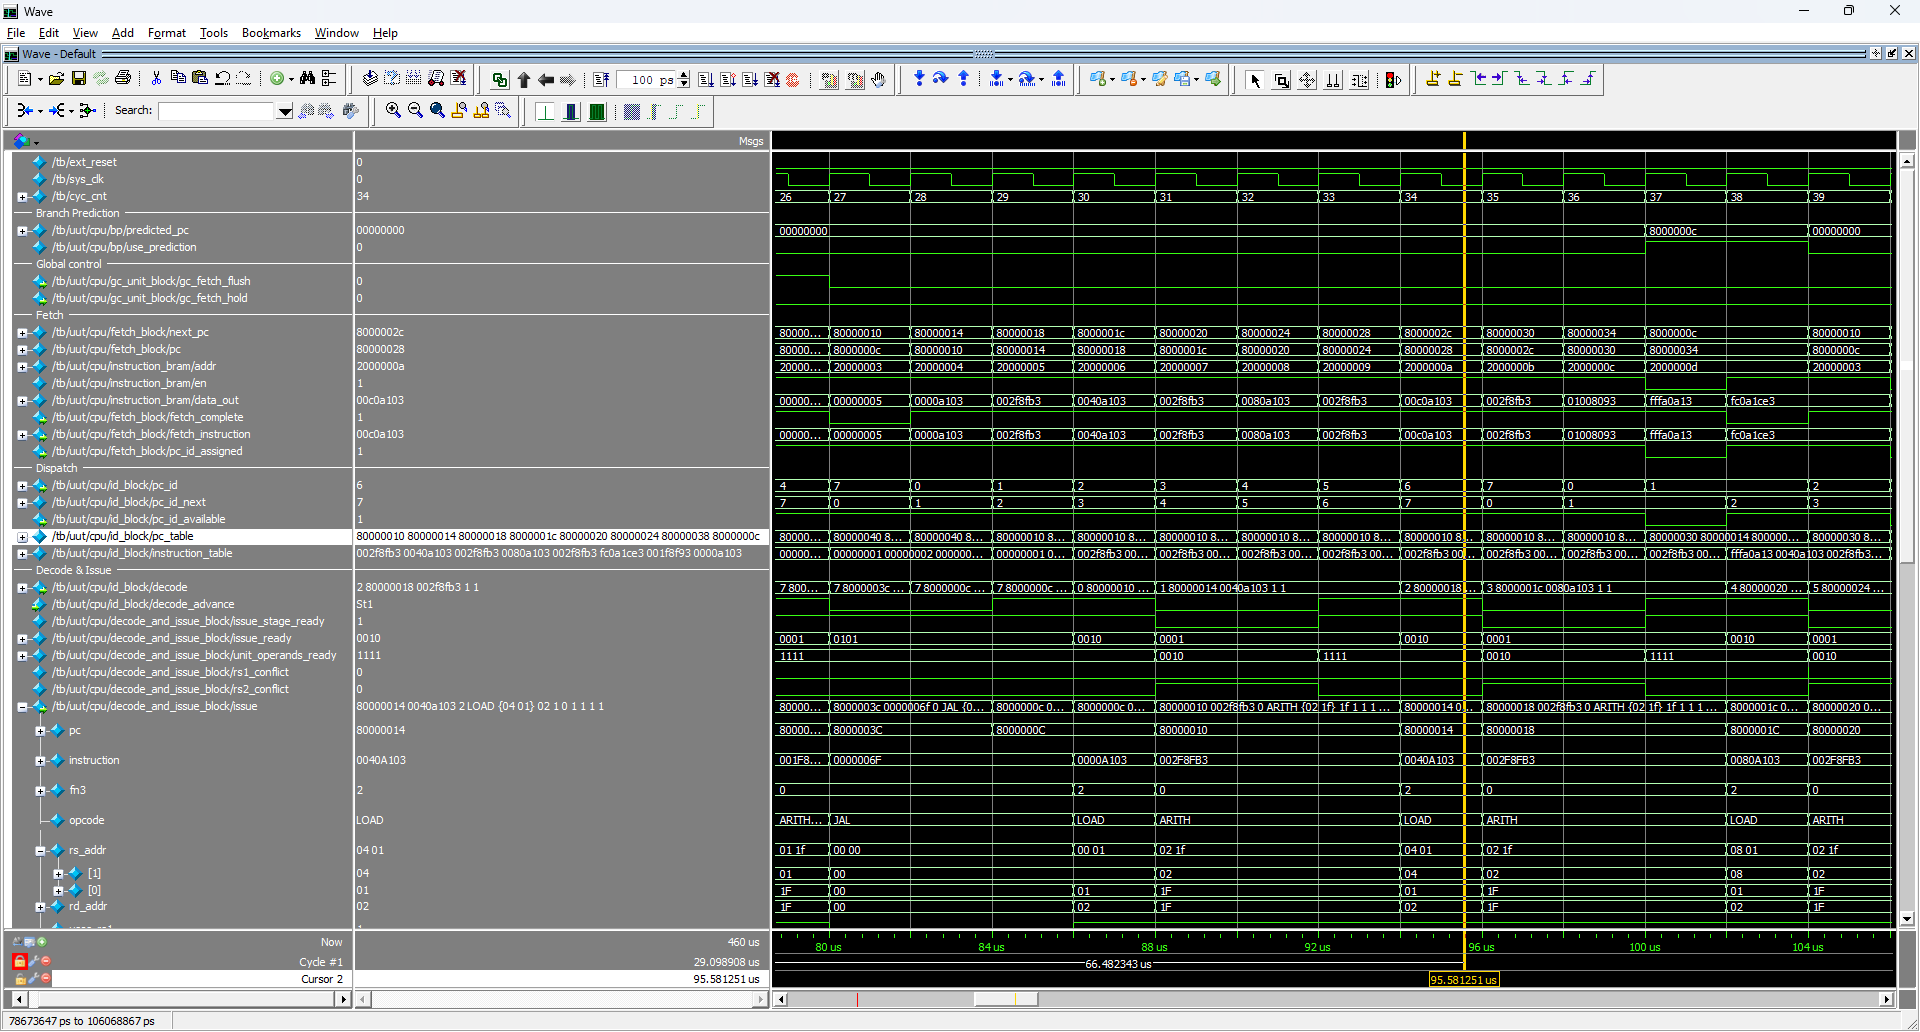
\includegraphics[scale=0.25]{images/03-D.png}
 \captionof{figure}{Временная диаграмма выполнения стадии декодирования и планирования на выполнение \textbf{команды 8000002с на 2-й итерации}}
\end{center}
\mychapter{4}{Задание №4}

\begin{center}
\centering 
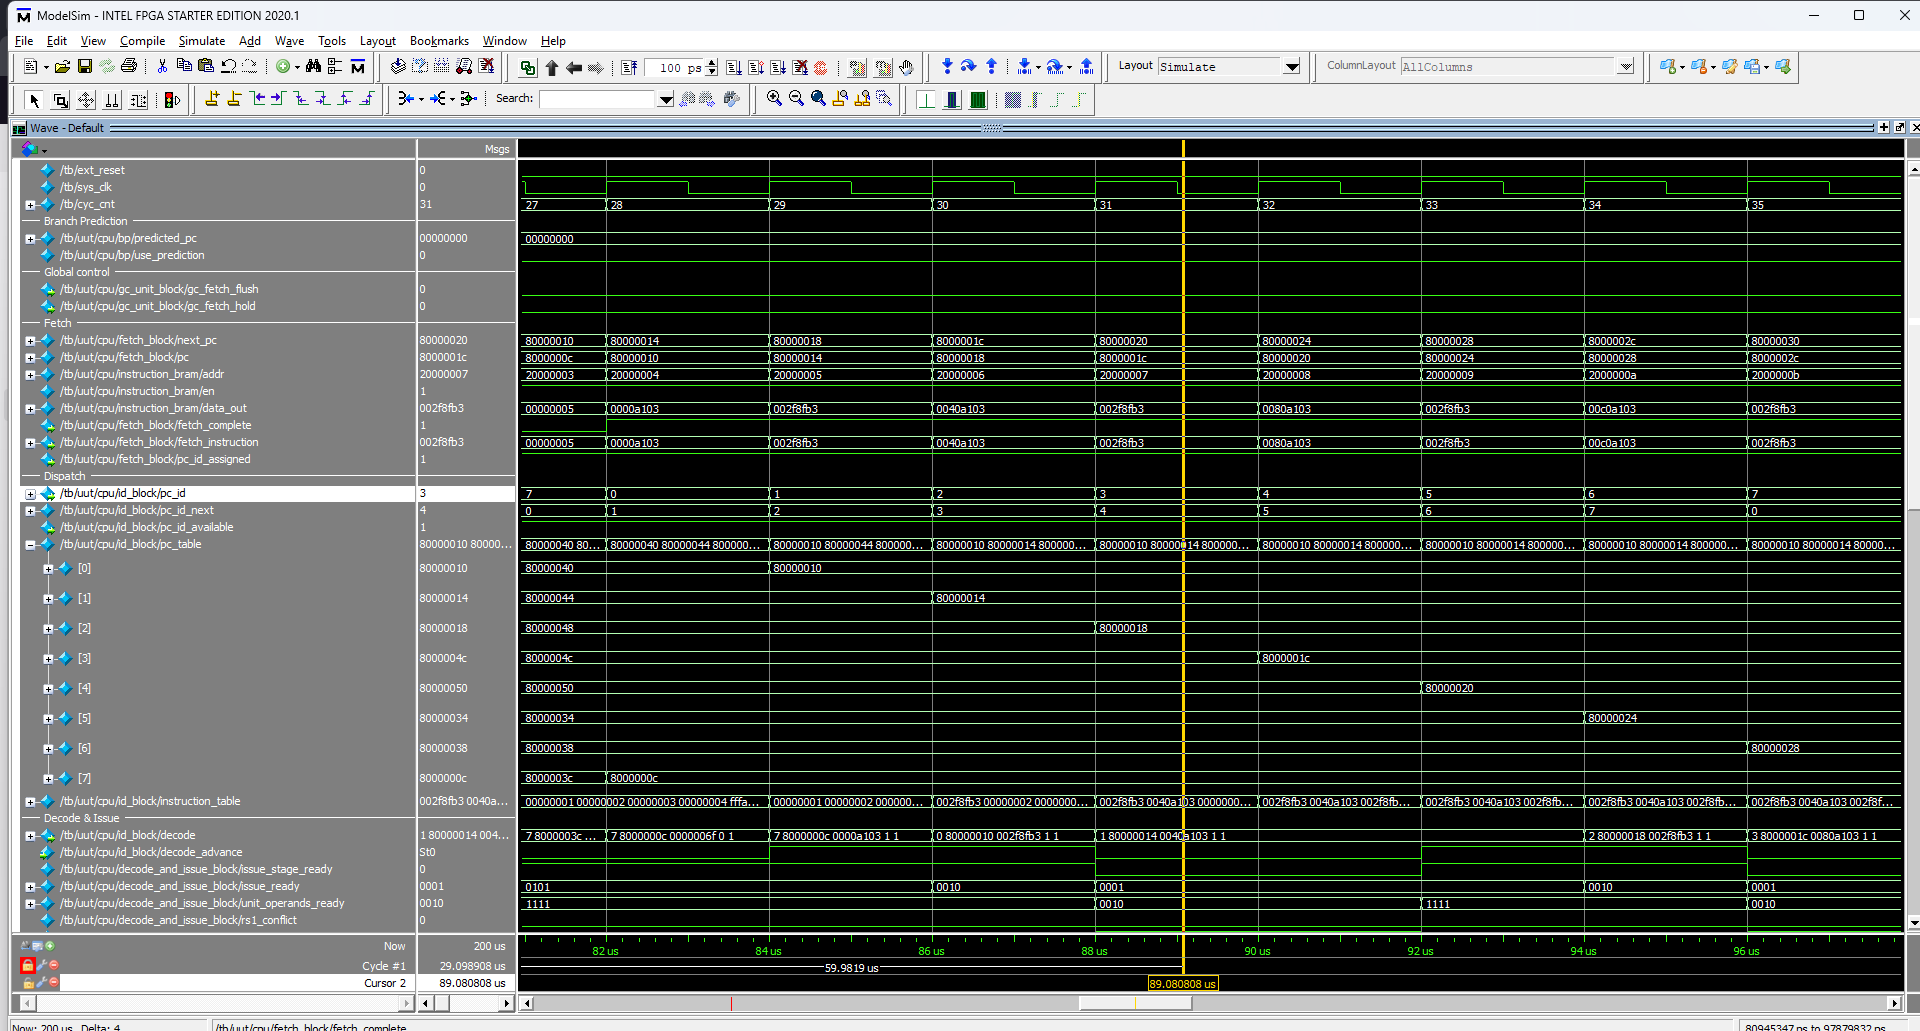
\includegraphics[scale=0.25]{images/04-F_ID.png}
 \captionof{figure}{Временная диаграмма команды add x31,x31,x2 2-ой итерации на стадии выборки и диспетчеризации}
\end{center}

\begin{center}
\centering 
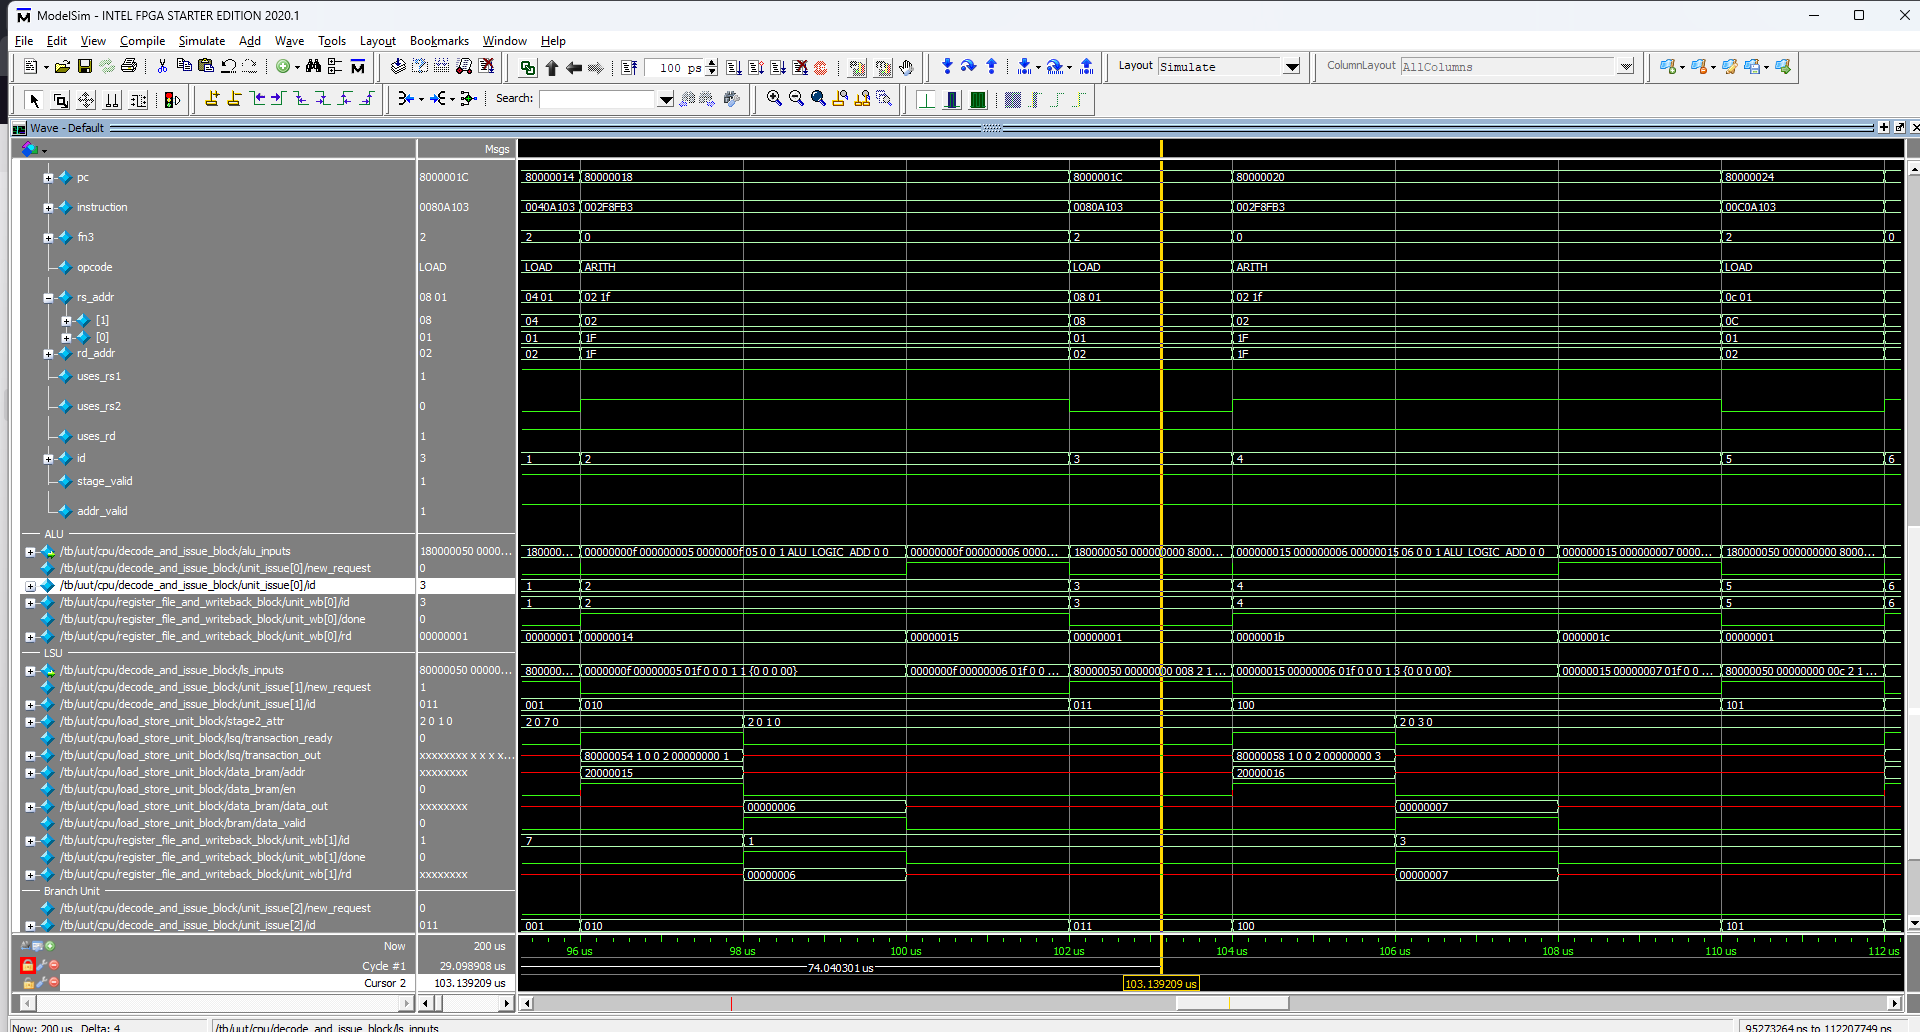
\includegraphics[scale=0.25]{images/04-AL.png}
 \captionof{figure}{Временная диаграмма команды add x31,x31,x2 2-ой итерации на стадии выполнения}
\end{center}
\mychapter{5}{Задание №5}

Значение регистра \textbf{x31} на момент окончания выполнения программы равно 9, как предполагалось ранее.

\begin{center}
\centering 
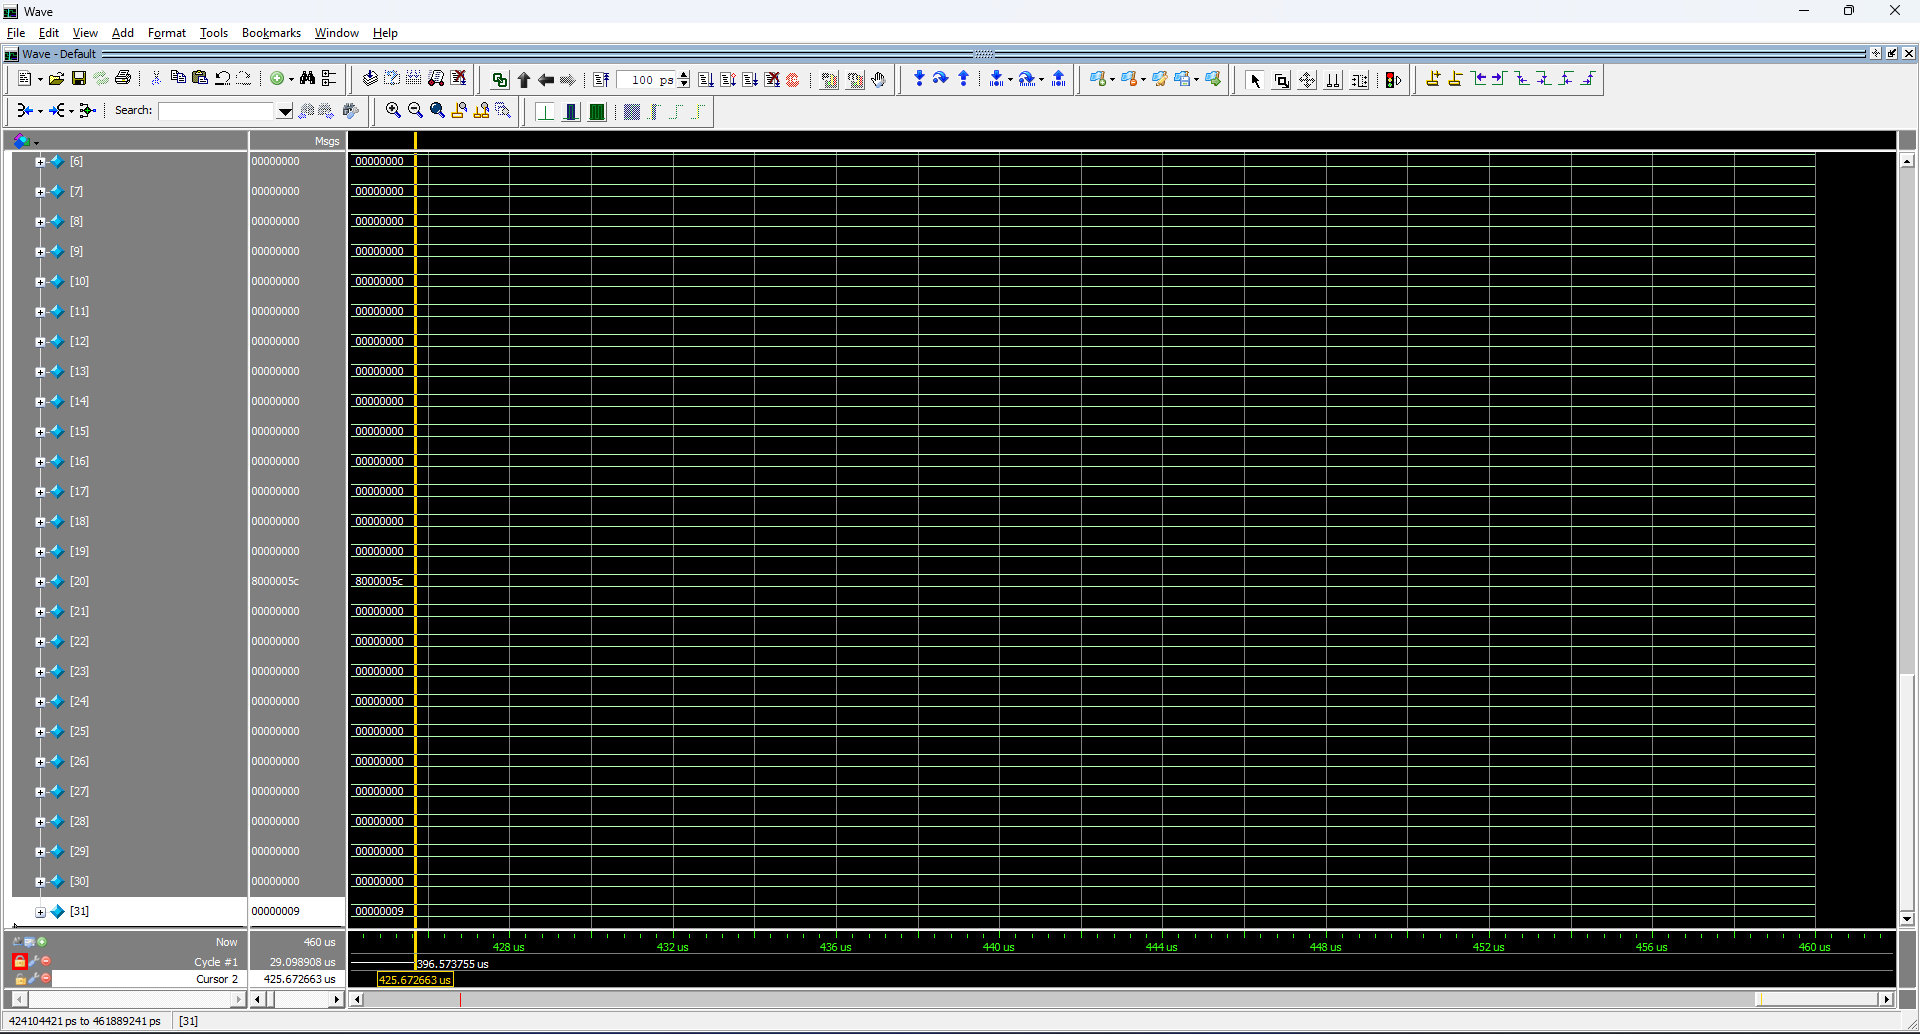
\includegraphics[scale=0.25]{images/05-x31_finally.png}
 \captionof{figure}{Значение регистра x31 на момент окончания выполнения программы}
\end{center}

\begin{center}
\centering 
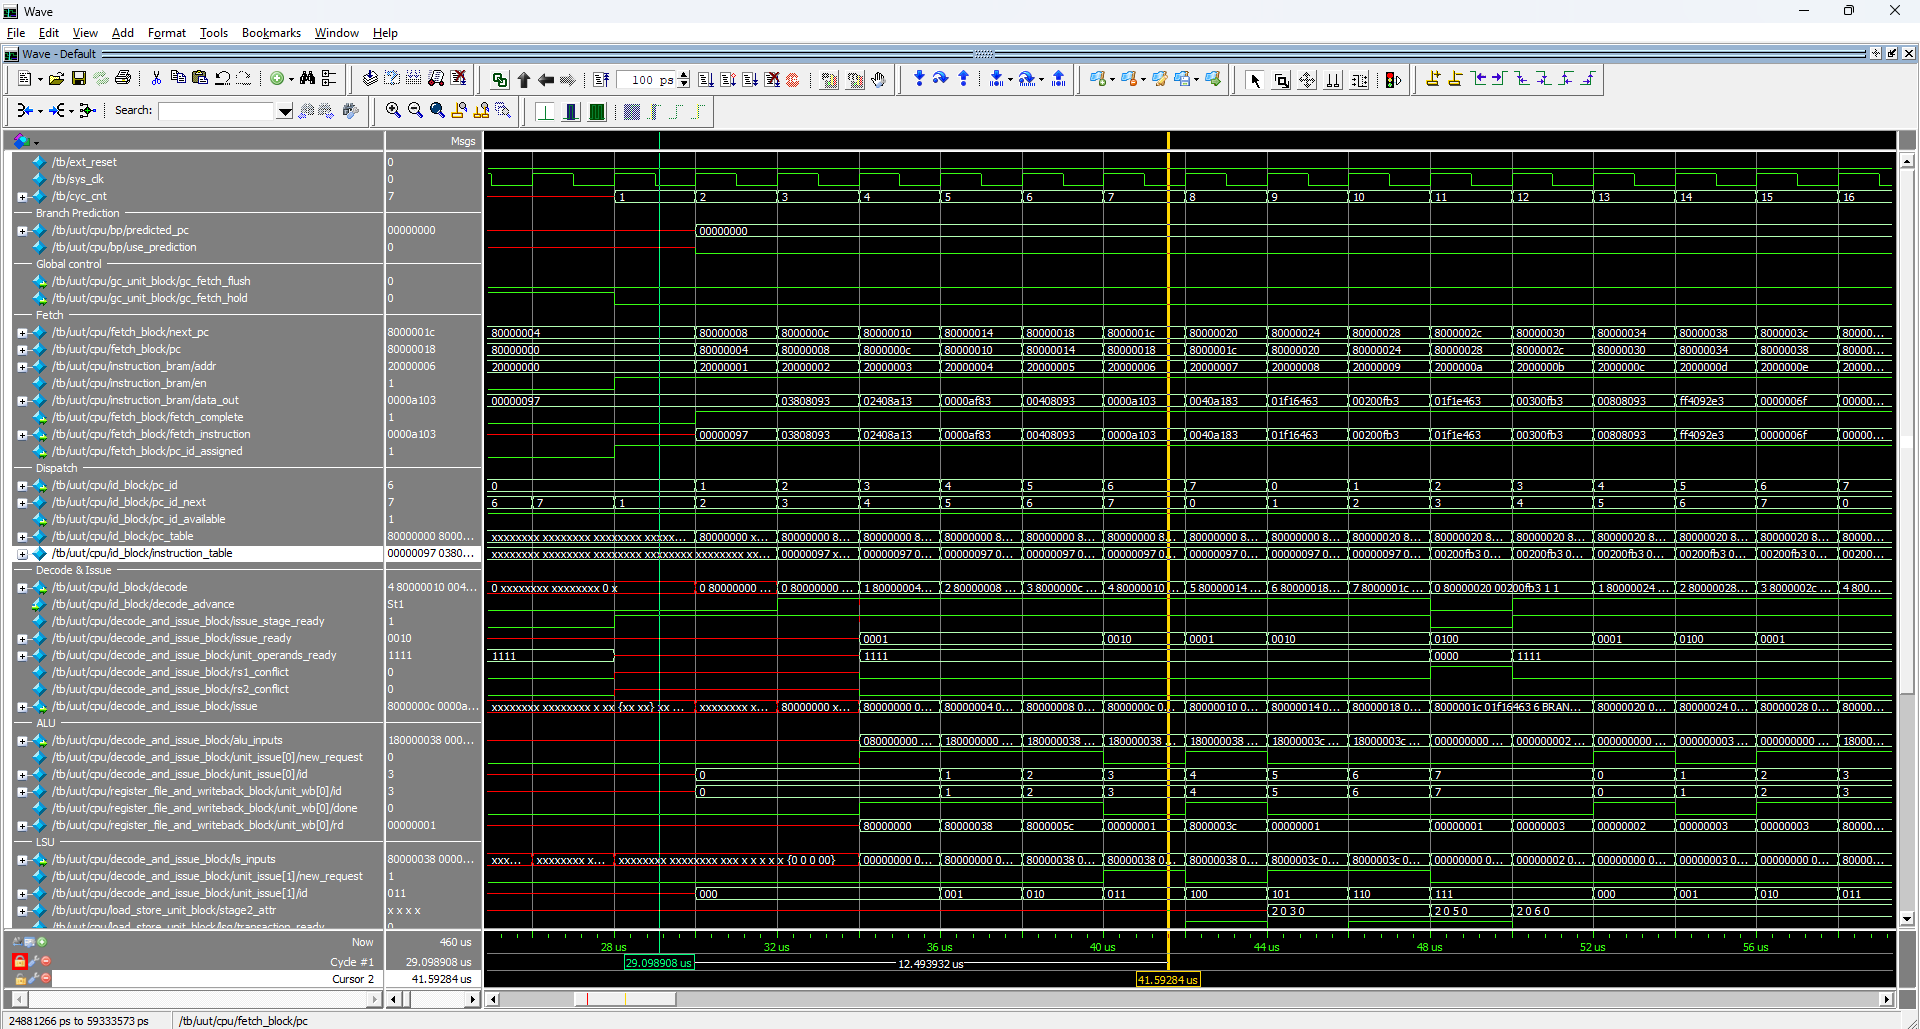
\includegraphics[scale=0.25]{images/05-fetch.png}
 \captionof{figure}{Временная диаграмма сигналов команды lw x3, 4(x1) на стадии выборки и диспетчеризации}
\end{center}

\begin{center}
\centering 
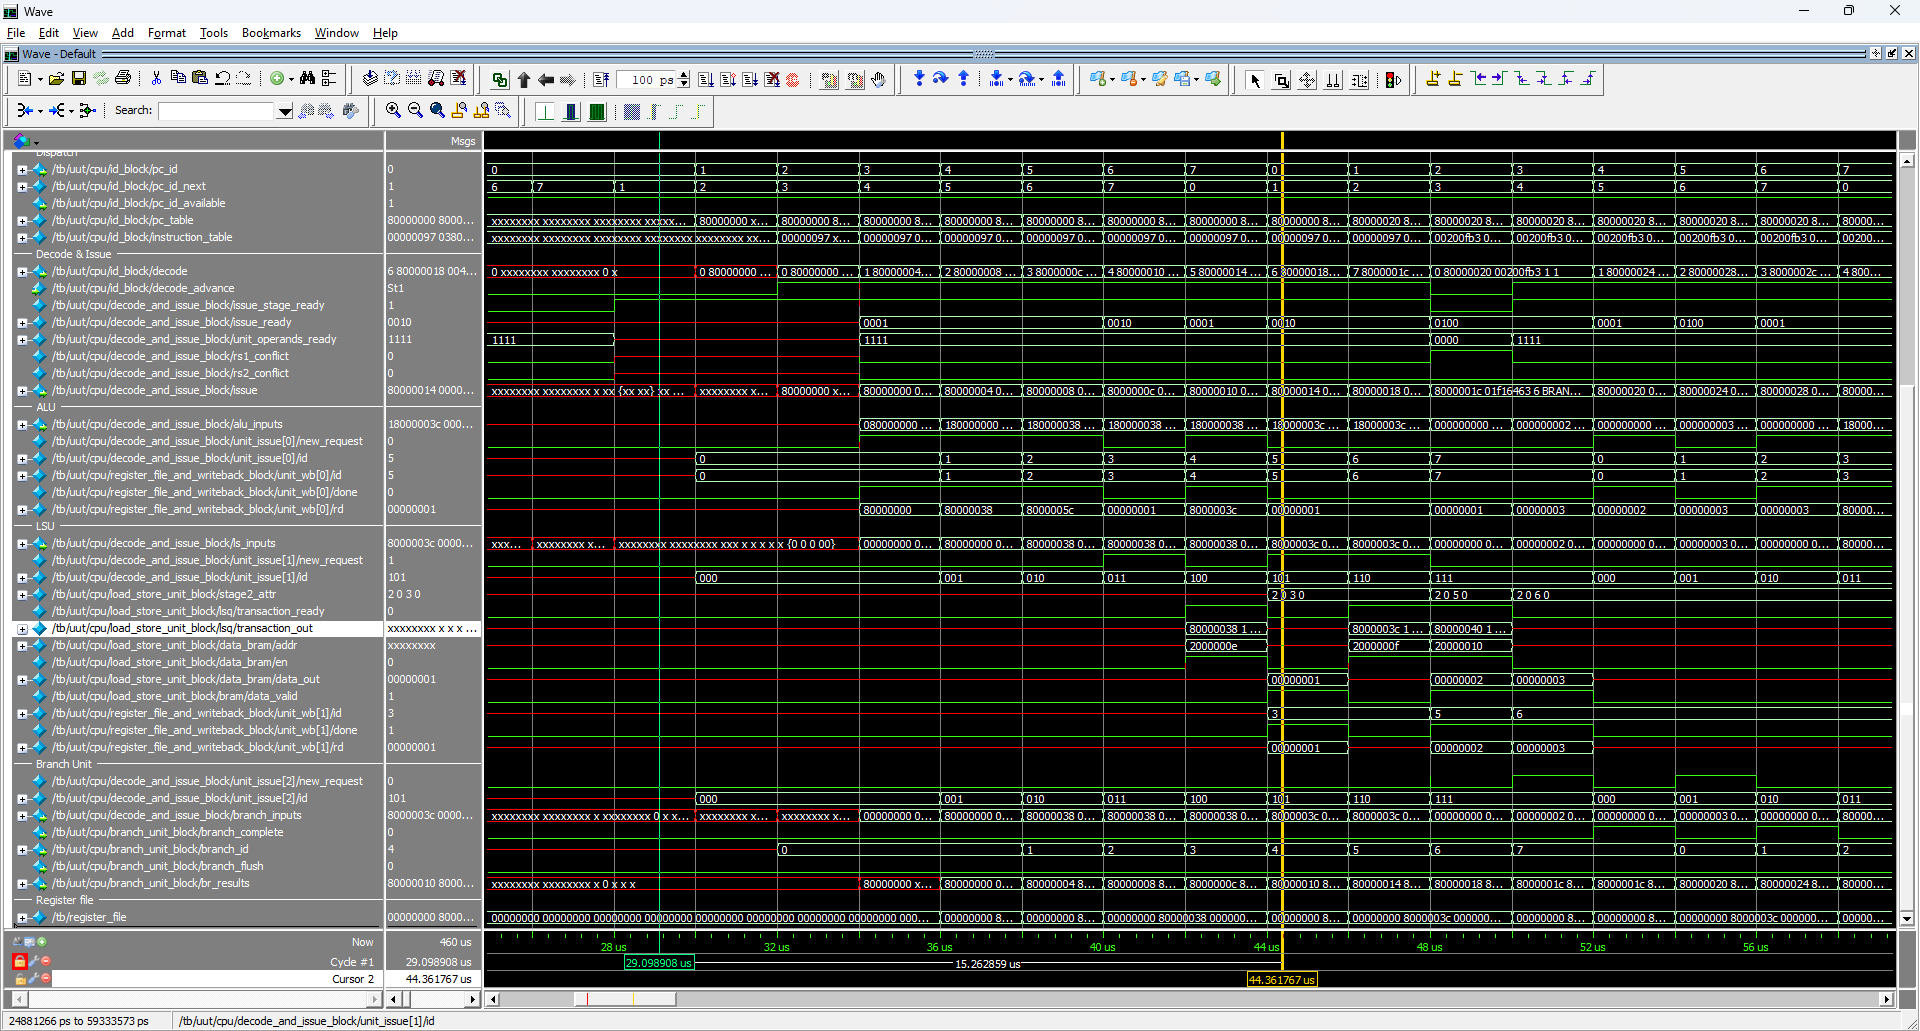
\includegraphics[scale=0.25]{images/05-decode.png}
 \captionof{figure}{Временная диаграмма сигналов команды lw x3, 4(x1) на стадии декодирования}
\end{center}

\begin{center}
\centering 
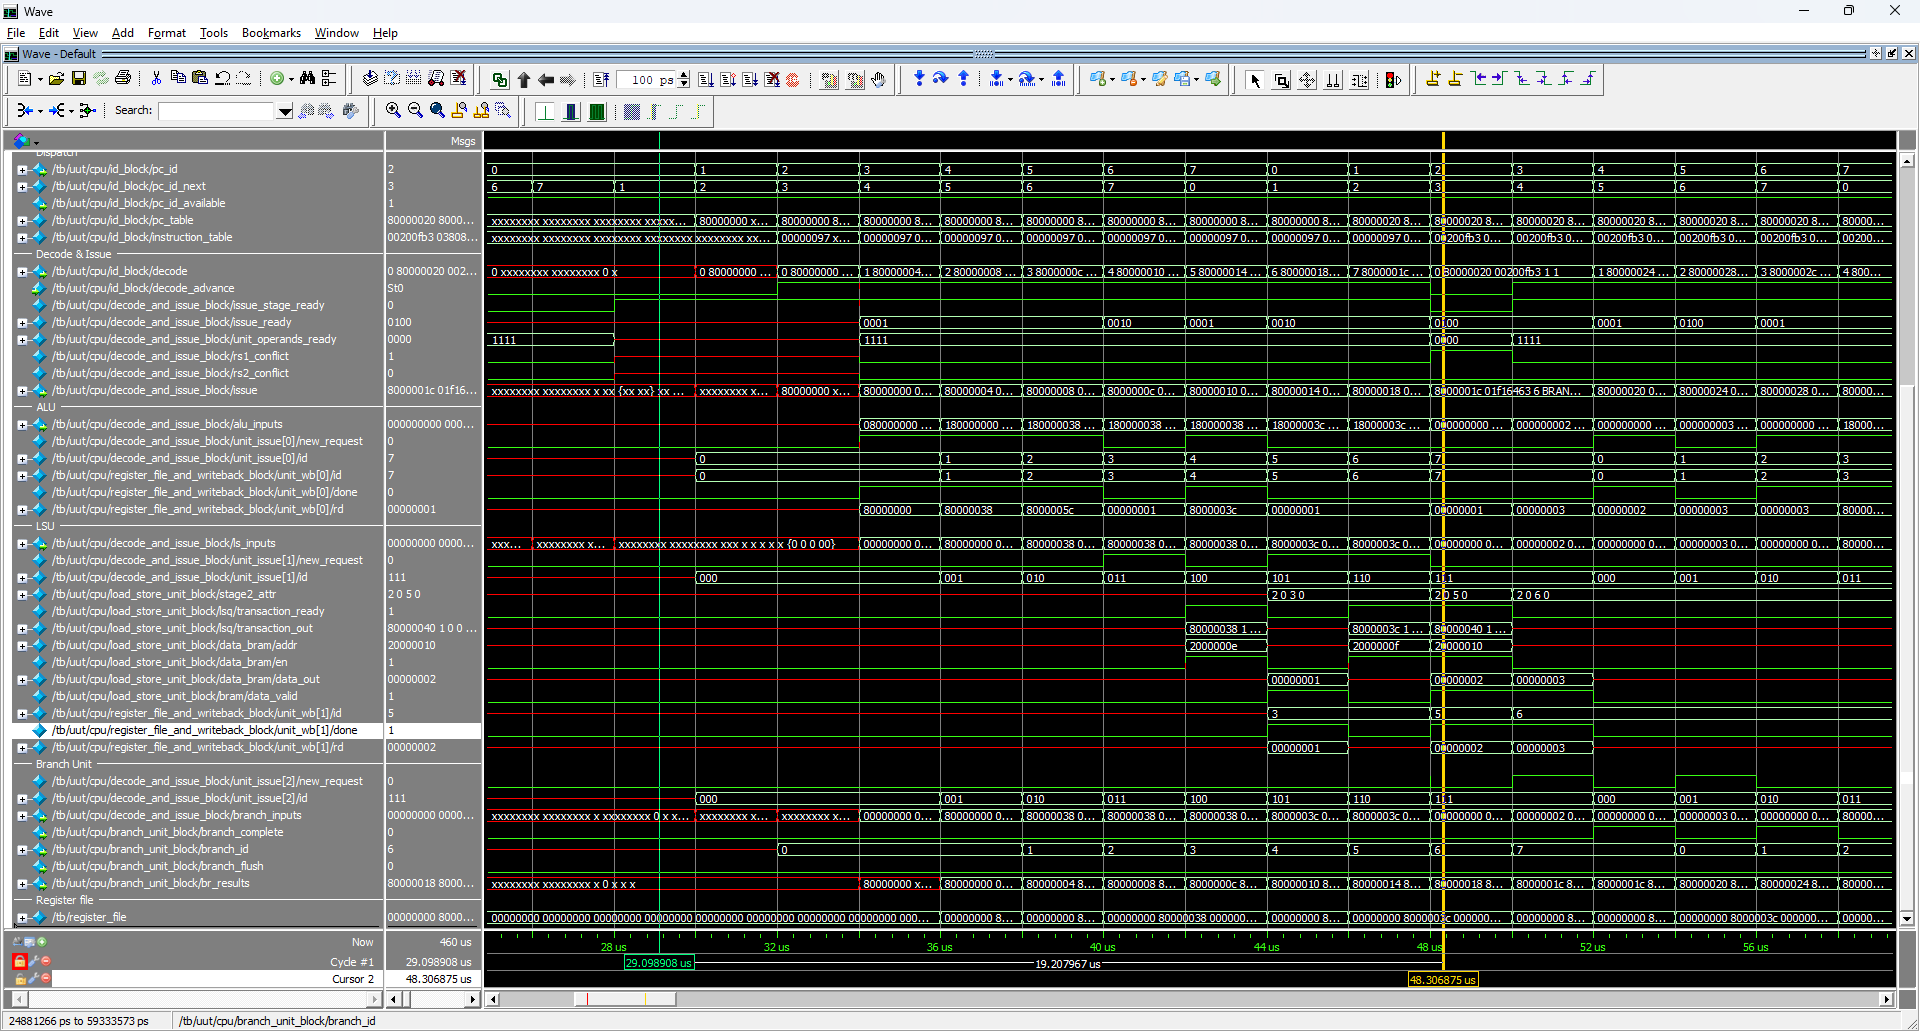
\includegraphics[scale=0.25]{images/05-execute.png}
 \captionof{figure}{Временная диаграмма сигналов команды lw x3, 4(x1) на стадии выполнения}
\end{center}

Программа достаточно хорошо оптимизирована, так как планирование производилось более чем на 75\% тактах. Если же попробовать, к примеру, поменять в цикле порядок загрузки значения в регистр и ветвления, то эффективность программы снизится.

\begin{center}
\centering 
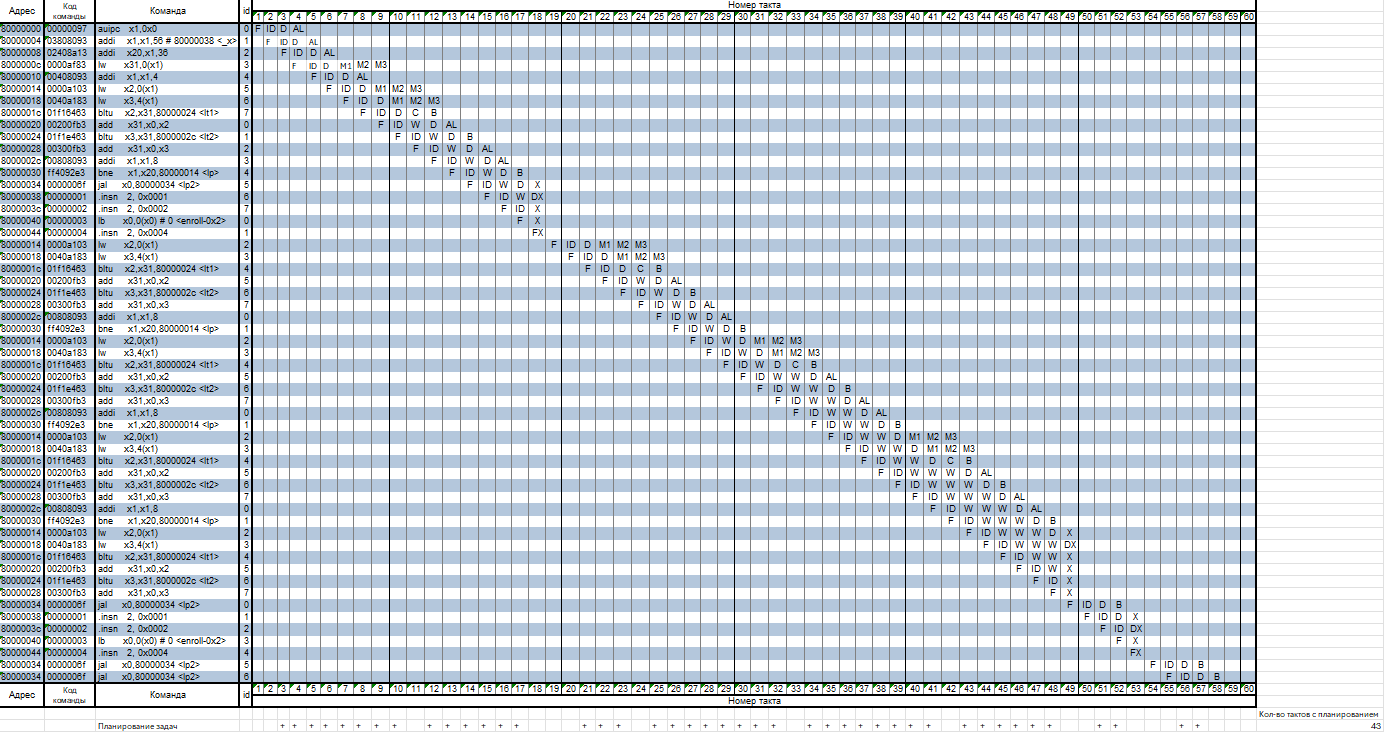
\includegraphics[scale=0.35]{images/05-route.png}
 \captionof{figure}{Трасса работы программы}
\end{center}

\makebibliography

\include{09-appendix}

\end{document}